\documentclass[a4paper]{article}

\usepackage{listings}
\usepackage{color}
\usepackage{todonotes}
\usepackage{enumerate}%used for custom enumerates
\usepackage{amssymb}
\usepackage{amsmath}
\usepackage{multicol}
%Colors for the listings
\definecolor{dkgreen}{rgb}{0,0.6,0}
\definecolor{gray}{rgb}{0.5,0.5,0.5}
\definecolor{mauve}{rgb}{0.58,0,0.82}
%style setup for the listings
\lstset{frame=tb,
  language=Java,
  aboveskip=3mm,
  belowskip=3mm,
  showstringspaces=false,
  columns=flexible,
  basicstyle={\small\ttfamily},
  numbers=none,
  numberstyle=\tiny\color{gray},
  keywordstyle=\color{blue},
  commentstyle=\color{dkgreen},
  stringstyle=\color{mauve},
  breaklines=true,
  breakatwhitespace=true
  tabsize=3
}

\newcommand{\inline}[1]{\lstinline!#1!}%Inline code



\begin{document}
\section{Course Overview}
\begin{itemize}
\item Even though Moore's Law\footnote{``The number of transistors on integrated circuits doubles approximately every two years''} is still valid, heat and power are of primary concerns. 
\begin{itemize}
\item These challenges can be overcome with smaller and more efficient processors or simply more processors
\item To make better use of the added computation power, parallelism is used.
\end{itemize}
\item Parallel vs. Concurrent: In both cases, one of the difficulties is to actually determine which processes can overlap and which can't:
\begin{itemize}
\item Concurrent: Focus on which activities may b executed at the same time (= overlapping execution)
\item Parallel: Overlapping execution on a real system with constraints imposed by the execution platform.
\end{itemize}
\item Parallel/Concurrent vs. distributed: In addition to parallelism/concurrency, systems can actually be physically distributed (e.g. BOINC)
\item Concerns in PP:
\begin{itemize}
\item Expressing Parallelism
\item Managing state (data)
\item Controlling/coordinating parallel tasks and data
\end{itemize}
\end{itemize}

\section{Parallel Architectures}
\begin{itemize}
\item Turing machine:
\begin{itemize}
\item Infinite tape
\item Head that reads/writes symbols on tape
\item State registers
\item Program is expressed as rules: (reg)(head) $\to$ (reg)(head)(movement)
\end{itemize}
\item Today's computers: 
\begin{itemize}
\item Consist of CPU, memory and I/O
\item Stored Program: program instructions are stored in memory
\item Von Neumann Architecture: Program data and program instruction in the same memory
\end{itemize}
\item Since accessing memory became slower than accessing CPU registers, CPUs now have caches which are closer (faster and smaller) to the CPU. Caches are:
\begin{itemize}
\item Faster then memory
\item Smaller than memory
\item Organized in multi-level hierarchies (e.g. L1,L2,L3)
\end{itemize}
\item To improve sequential processor performance, you can use the following parallelism techniques:
\begin{itemize}
\item Vectorization\\
For example, when adding vectors (load $\to$ operation(s) $\to$ store)
\begin{itemize}
\item Normal: 1-at-a-time
\item Vectors: N-at-a-time (bigger registers)
\end{itemize}
\item Pipelining\footnote{Think laundry: you can either wash, dry, fold and repeat, or while the $n$ load is drying, the $n+1$ load can start washing}\todo[inline]{maybe add diagram from slides?}
\begin{itemize}
\item Multiple stages (CPU Functional Units)
\begin{itemize}
\item Instruction Fetch
\item Instruction Decode
\item Execution
\item Data access
\item Writeback
\end{itemize}
\item Each instruction takes 5 time units (cycles)
\item 1 instruction per cycle (not always possible though)
\end{itemize}
\item Instruction Level Parallelism (ILP)
\begin{itemize}
\item Superscalar CPUs
\begin{itemize}
\item Multiple instructions per cycle
\item multiple functional units
\end{itemize}
\item Out-of-Order (OoO) Execution
\begin{itemize}
\item Potentially change execution order of instructions
\item As long as the programmer observes the sequential program order
\end{itemize}
\item Speculative execution
\begin{itemize}
\item Predict results to continue execution
\end{itemize}
\end{itemize}
\end{itemize}
\item Moore's Law
\begin{itemize}
\item\emph{``The number of transistors on integrated circuits doubles approximately every two years''} - Gordon E.Moore, 1965
\item Actually an observation
\item For a long time, CPU Architects improved sequential execution by exploiting Moore's Law and ILP
\item More transistors $\to$ more performance
\item Sequential programs were becoming exponentially faster with each new CPU
\begin{itemize}
\item (most) programmers did not worry about performance
\item They waited for the next CPU model
\end{itemize}
\end{itemize}
\item Architects hit walls 
\begin{itemize}
\item Power dissipation wall: Making CPU faster $\to$ expensive to cool
\item Memory Wall: CPUs faster than memory access
\item ILP Wall: Limits in inherent program's ILP, complexity
\item \textbf{No longer affordable to increase sequential CPU performance}
\end{itemize}
\item Multicore processors
\begin{itemize}
\item Use transistors to add cores (instead of improving sequential performance)
\item Expose parallelism to software
\item Implication: Programmers need to write parallel programs to take advantage of new hardware
\begin{itemize}
\item Past: Parallel programming was performed by a few
\item Now: Programmers need to worry about (parallel) performance
\end{itemize}
\end{itemize}
\item Shared memory architectures \todo[inline]{Maybe add picture form slides, page 34 form 2 - parallel architectures; ADD PICTURES FOR EACH OF THE DIFFERENT TYPES OF SMA}
\begin{itemize}
\item SMT (Hyperthreading)
\begin{itemize}
\item Single core
\item Multiple instruction streams (threads); Virtual (phony) cores
\item Between ILP $\leftrightarrow$ multicore
\begin{itemize}
\item ILP: Multiple units for one instruction stream
\item SMT: Multiple units for multiple instruction streams
\end{itemize}
\item Limited parallel performance
\end{itemize}
\item Multicores
\begin{itemize}
\item Single chip, multiple cores
\item Dual-, Quad-, x8\dots
\item Each core has its own hardware units; computations un parallel perform well
\item Might share part of the cache hierarchy
\end{itemize}
\item SMP (Symmetric MultiProcessing)
\begin{itemize}
\item Multiple CPUs on the same system
\item CPUs share memory: same cost to access memory
\item CPU caches coordinate: Cache coherence protocol
\end{itemize}
\item NUMA (Non-Uniform Memory Access)
\begin{itemize}
\item Memory is distributed
\item Local/Remote (fast/slow)
\item Shared memory interface
\end{itemize}
\end{itemize}
\item Flynn's Taxonomy 
\todo[inline]{Add diagram from page 49 of 2 - parallel architectures}
\item GPUs
\begin{itemize}
\item Graphical Processing Units 
\begin{itemize}
\item Scene description $\to$ pixels
\item Highly data-parallel process
\end{itemize}
\item Massively parallel vector machines
\item Not a standard component up until recently
\item Started very specialized (rigid pipelines)
\item Driven by game industry success
\end{itemize}
\item GP-GPUs
\begin{itemize}
\item General programming using GPUs (CUDA, OpenCL)
\item Much research on ``how to execute X on a GPU''
\item Generally GPUs are:
\begin{itemize}
\item Well suited for data parallel programs
\item Not very well-suited for programs with random accesses
\item People are rethinking algorithms
\end{itemize}
\item GPUs are, currently, something of a standard in the HPC (High Performance Computing) domain
\end{itemize}
\end{itemize}

\section{Basic Concepts}
\begin{itemize}
\item Performance in sequential execution:
\begin{itemize}
\item Computational complexity
\begin{itemize}
\item Theoretical computer science
\item Asymptotic behavior: big O notation ($\mathcal{O}$), or big $\Theta$
\item How many steps does an algortithm take
\item Complexity classes
\end{itemize}
\item Execution Time: The less time, the better
\end{itemize}
\item Sequential programs are much easier to write, but if we care about performance we have to write parallel programs
\item Parallel Performance
\begin{itemize}
\item Sequential execution time: $T_1$
\item Execution time $T_p$ on $p$ CPUs:
\begin{itemize}
\item $T_p=\frac{T_1}{p}$ (Perfection)
\item $T_p>\frac{T_1}{p}$ (Performance Loss, what normally happens)
\item $T_p<\frac{T_1}{p}$ (Sorcery!)
\end{itemize}
\end{itemize}
\item (Parallel) Speedup
\begin{itemize}
\item (Parallel) speedup $S_p$ on $p$ CPUs: \[S_p=\frac{T_1}{T_p}\]
\begin{itemize}
\item $S_p=p\to$ linear speedup (Perfection)
\item $S_p<p\to$ sublinear speedup (Performance loss)
\item $S_p>p\to$ superlinear speedup (Sorcery!)
\end{itemize}
\item Efficiency: $\frac{S_p}{p}$
\end{itemize}
\item Scalability: How well a system reacts to increased load 
\begin{itemize}
\item In Parallel Programming
\begin{itemize}
\item Speedup when we increase processors
\item What will happen if number of processors $\to\infty$
\end{itemize}
\end{itemize}
\item Performance loss ($S_p<p$) happens because:
\begin{itemize}
\item Programs may not contain enough parallelism, e.g.:
\begin{itemize}
\item pipeline with 4 stages on a 32-CPU machine
\item Some parts of the program might be sequential
\end{itemize}
\item Overheads introduced by parallelization; typically associated with coordination
\item Architectural limitations, e.g. memory contention
\end{itemize}
\item Amdahl's Law
\begin{itemize}
\item $b$: sequential part (no speedup)
\item $1-b$: parallel part (linear speedup)
\end{itemize}
\[{T_p} = {T_1}\left( {b + \frac{{1 - b}}{p}} \right)\hspace{10mm}{S_p} = \frac{p}{{1 + b\left( {p - 1} \right)}}\]
\begin{itemize}
\item Remarks About Amdahl's Law:
\begin{itemize}
\item It concerns maximum speedup (Optimistic approach). Architectural constrains will make factors worse
\item Takeaway: \textbf{All non-parallel parts of a program (no matter how small) can cause problems!}
\item Law of diminishing returns\footnote{The law of diminishing returns (also law of diminishing marginal returns or law of increasing relative cost) states that in all productive processes, adding more of one factor of production, while holding all others constant, will at some point yield lower per-unit returns [Taken from Wikipedia]}
\end{itemize}
\end{itemize}
\item Gustafson's Law
\begin{itemize}
\item An Alternative (optimistic) view to Amdahl's Law
\item Observations:
\begin{itemize}
\item Consider problem size
\item Run-time, not problem size, is constant
\item More processors allows to solve larger problems in the same time
\item Parallel part of a program scales with the problem size
\end{itemize}
\item Formula:
\begin{itemize}
\item $b$: sequential part (no speedup)
\begin{align*}
T_1&=p(1-b)T_p+bT_p\\
S_p&=p-b(p-1)
\end{align*}
\end{itemize}
\end{itemize}
\item Concurrency vs. Parallelism
\begin{itemize}
\item Concurrency is:
\begin{itemize}
\item A programming model
\item Programming via independently executing tasks
\item About structuring a program 
\item A concurrent program does not have to be parallel
\end{itemize}
\item Parallelism:
\begin{itemize}
\item About execution
\item Concurrent programming is suitable for parallelism
\end{itemize}
\end{itemize}
\todo[inline]{Add views of different architectures} 
\item Concerns in Parallel programming
\begin{itemize}
\item Expressing parallelism
\begin{itemize}
\item Work partitioning (Split up work for a single program into parallel tasks). Can be done:
\begin{itemize}
\item Manually (task parallelism): User explicitly expresses tasks
\item Automatically by the system (e.g. in data parallelism): User expresses an operation and the system takes care of how to split it up 
\end{itemize}
\item Scheduling
\begin{itemize}
\item Assign task to processors (usually done by the system)
\item goal: full utilization (no processor is ever idle)
\end{itemize}
\end{itemize}
\item Managing state (data)
\begin{itemize}
\item Shared vs. distributed memory architectures (in the latter, data needs to be distributed)
\item Which parallel tasks access which data, and how (e.g. READ or WRITE access)
\item (Potentially) split up data. Ideal: each task exclusively accesses its own data
\item Depending on the application:
\begin{itemize}
\item Tasks, then data
\item Data, then tasks
\end{itemize}
\end{itemize}
\item Controlling/Coordinating parallel tasks and data
\begin{itemize}
\item Distributed data
\begin{itemize}
\item No coordination (e.g. embarrassingly parallel)
\item Messages
\end{itemize}
\item Shared data: controlling concurrent access
\begin{itemize}
\item Concurrent access may cause inconsistencies
\item Mutual exclusion to ensure data consistency
\end{itemize}
\end{itemize}
\end{itemize}
\item Coarse vs. Fine Granularity
\begin{itemize}
\item Fine granularity
\begin{itemize}
\item More portable (can be executed in machines with more processors)
\item Better for scheduling 
\item Parallel slackness (Expressed parallelism >> machine parallelism)
\item BUT: if scheduling overhead is comparable to a single task $\to$ overhead dominates
\end{itemize}
\item Guidelines:
\begin{itemize}
\item As small as possible
\item but, significantly bigger than scheduling overhead; system designers strive to make overheads small
\end{itemize}
\item Coordinating tasks:
\begin{itemize}
\item Enforcing ordering between tasks, e.g.:
\begin{itemize}
\item Task X uses result of task A
\item Task X needs to wait for task A to finish
\end{itemize}
\item Example primitives:
\begin{itemize}
\item \emph{barrier}
\item \emph{send()/receive()}
\end{itemize}
\item All tasks need to reach the barrier before they can proceed
\end{itemize}
\end{itemize}
\end{itemize}

\section{Parallel programming models}
\begin{itemize}
\item Parallel Programming is not uniform
\begin{itemize}
\item Similar to sequential programming
\item Many different approaches to solve problems
\item Many are equivalent under certain conditions, it depends on the application
\item More of an art than a science
\end{itemize}
\item Task Parallel: Programmer explicitly defines parallel tasks (generic, not always productive)
\begin{itemize}
\item Tasks:
\begin{itemize}
\item Execute code
\item Spawn other tasks
\item wait for results from other tasks
\end{itemize}
\item A graph is formed based on spawning tasks\\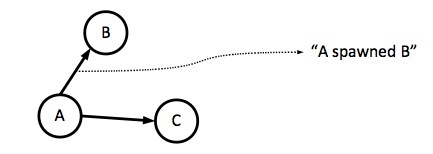
\includegraphics[scale=0.5]{Figures/chapter4slide7.jpg}
\item Example: Fibonacci function 
\begin{lstlisting}
public class Fibonacci {
   public static long fib(int n) {
      if (n < 2)
         return n;
      spawn a task to execute fib(n-1);
      spawn a task to execute fib(n-2);
      wait for the tasks to complete
      return the addition of the task results
      } 
}
\end{lstlisting}
\item Tasks can execute in parallel
\begin{itemize}
\item But they don't have to
\item Assignment of tasks to CPU is up to the scheduler
\end{itemize}
\item Task graph is dynamic: unfolds as execution proceeds
\item Intuition: wide task graph $\to$ more parallelism
\item Time:\todo[inline]{Check for a better explanation somewhere else}
\item Scheduling
\begin{itemize}
\item algorithm for assigning tasks to processors
\item There exists a scheduling with
\[T_p\leq \frac{T_1}{p}+T_\infty\] 
\item This upper bound can be achieved with a greedy scheduler
\begin{enumerate}
\item if $\geq p$ tasks exist, $p$ tasks execute
\item if $< p$ tasks exist, all execute
\end{enumerate}
\item optimal with a factor of 2
\item linear speedup for $\frac{T_1}{T_\infty}\geq P$
\end{itemize}
\item Work stealing scheduler
\begin{itemize}
\item First used in CIlk
\item provably: $T_p=\frac{T_1}{P}+O\left( T_\infty\right)$
\item empirically: $T_p\approx\frac{T_1}{P}+T_\infty$
\item $\frac{T_1}{T_\infty}>>P\to$ linear speedup
\item Parallel slackness: granularity
\item Why should the programmer care? A: guideline for parallel programs
\end{itemize}
\item Example: Sum the elements of a list, using D\&C\footnote{D\&C: Divide and Conquer}
\begin{lstlisting}
public static long sum_rec(List<Long> Xs){
    int size = Xs.size();
    if (size == 1)
        return Xs.get(0);
    int mid = size / 2;
    long sum1 = sum_rec(Xs.subList(0, mid)); 
    long sum2 = sum_rec(Xs.subList(mid, size)); 
    return sum1 + sum2;
}
\end{lstlisting}
\begin{lstlisting}
Divide and Conquer:
    if cannot divide:
        return unitary solution (stop recursion)
    divide problem in two
    solve first (recursively)
    solve second (recursively)
    combine solutions
    return result
\end{lstlisting}
\item So far: Dynamic task graph, but the graph can also be static, i.e. does not change with time
\begin{itemize}
\item Pipeline
\begin{itemize}
\item Think Laundry as an example
\item In full utilization, output rate is 1 item per time unit
\item Time unit is determined by the slower stage: a slower stage stalls the pipeline
\item Hence, we try to create pipelines where each stage takes (roughly) the same amount of time
\item Achieved using splits and joins for parallel stages\\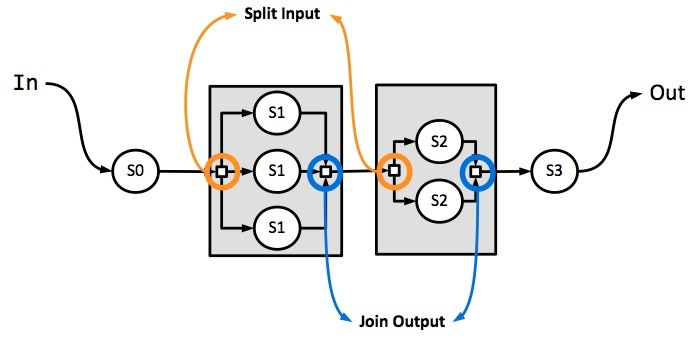
\includegraphics[scale=0.38]{Figures/chapter4slide30.jpg}
\end{itemize}
\item Streaming\todo[inline]{There isn't a single thing in the slides about streaming}
\item Dataflows
\begin{itemize}
\item Programmer defines: what each task does, and how the tasks are connected
\item Scheduling: Assigning nodes (tasks) into processors
\item $n<p$: cannot utilize all processors
\item $n == p$: one node per processor
\item $n>p$: need to combine tasks; portability, flexibility (parallel slackness); balancing, minimize communication (graph partitioning)
\item Dataflow programming is a good match for parallel programming since the programmer is not concerned with low-level details; and the same program is used for different platforms (e.g. shared/distributed memory $\to$ different edge impl.)
\end{itemize}
\end{itemize}
\end{itemize}
\item Data parallel: An operation is applied simultaneously to an aggregate of individual items (e.g. arrays) (productive, not general)
\begin{itemize}
\item In task parallelism, programmer describes what each task does and the task graph (dynamic or static)
\item In data parallelism, the programmer describes an operation on an aggregate of data items. 
\begin{itemize}
\item Data partitioning is done by the system
\item D.P. is declarative: programmer describes what, not how
\end{itemize}
\item Example: Map\\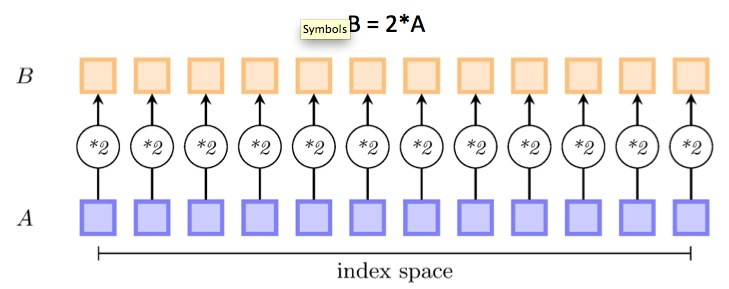
\includegraphics[scale=0.42]{Figures/chapter4slide34.jpg}
\begin{itemize}
\item Each operation can be performed in parallel
\item Work partitioning $\to$ partition the index space
\end{itemize}
\item Reductions
\begin{itemize}
\item Simple examples: sum, max
\item Reductions over programmer-defined operations
\begin{itemize}
\item Operation properties (associativity/commutativity) define the correct executions
\item Supported in most parallel languages/frameworks
\item powerful constru\todo{Word is chopped}
\end{itemize}
\item Other data types than arrays
\item similar operation: prefix scan
\end{itemize}
\item Parallel Loops
\begin{itemize}
\item So far: work partition $\to$ partition object (e.g. array) index space
\item Iterations can (but do not have to) perform in parallel: work partitioning $\to$ partition iteration space
\item Add generality
\item Potential source of bugs if thought of as a sequential loop due to data races
\end{itemize}
\end{itemize}
\item Managing State: Main challenge for parallel programs. There are different approaches:
\begin{itemize}
\item Immutability
\begin{itemize}
\item Data does not change
\item best option, should be used when possible
\end{itemize}
\item Isolated mutability
\begin{itemize}
\item Data can change, but only one execution context can access them
\item message passing for coordination
\item State is not shared
\item Each task (actor) holds its own state
\item (Asynchronous) messages
\item Models:
\begin{itemize}
\item Actors
\item Communicating Sequential processes (CSP)
\end{itemize}
\end{itemize}
\item Mutable/shared data
\begin{itemize}
\item Data can change/all execution contexts can potentially access them
\item Enabled in shared memory architectures
\begin{itemize}
\item \textbf{However}: concurrent accesses may lead to inconsistencies
\item \textbf{Solution}: protect state by allowing only one execution context to access it at a time
\end{itemize}
\item State needs to be protected
\begin{itemize}
\item Exclusive access
\item intermediate inconsistent states should not be observed\footnote{Think two people at the blackboard example}
\end{itemize}
\item Methods
\begin{itemize}
\item \textbf{Locks}: Mechanisms to ensure exclusive access/atomicity; ensuring good performance/correctness with locks can be hard
\item \textbf{Transactional Memory}: Programmer describes a set of actions that need to be atomic; easier for the programmer, but getting good performance might be challenging
\end{itemize}
\end{itemize}
\end{itemize}
\end{itemize}

\section{Introduction to (Parallel) Programming}
\todo[inline]{Not really needed??}

\section{Introduction to Java}
\todo[inline]{Only the technical things are discussed, no basic java syntax!}
\begin{itemize}
\item Java is an interpreted language
\begin{itemize}
\item Platform independence via bytecode interpretation
\item Java programs run (in theory) on any computing device (PC, mobile, linux, etc.)
\item Java compiler translates source to byte code
\item Java Virtual Machine (JVM) interprets compiled program
\end{itemize}
\item Compiling/Running
\begin{enumerate}
\item Write it
\begin{itemize}
\item Code or source code: The set of instructions in a program
\end{itemize}
\item Compile it
\begin{itemize}
\item Compile: Translate a program from one language to another
\item Byte code: The java compiler converts your code into a format named \emph{byte code} that runs on many computer types
\end{itemize}
\item Run (execute) it
\begin{itemize}
\item Output: The messages printed to the user by a program
\end{itemize}
\end{enumerate}
\item JVM Bytecode interpretation
\begin{itemize}
\item JVM interprets compiled Bytecode
\item Simulates a virtual CPU (or rather an entire machine)
\item Translates bytecode into architecture dependent machine code at runtime
\item Loss in performance due to interpretation?
\begin{itemize}
\item Yes and no
\item Some overhead due to interpretation step but JVM is highly optimized
\item Other language constructs impact performance more
\end{itemize}
\end{itemize}
\item Structure of a Java program
\begin{lstlisting}
public class name {
	public static void main(String[] args){
		statement;
		statement;
		...
		statement;
	}
}
\end{lstlisting}
Where:
\begin{itemize}
\item \textbf{class}: a program
\item\textbf{method} (\inline{main}): a named group of statements
\item \textbf{statement}: a command to be executed
\end{itemize}
Also:
\begin{itemize}
\item \inline{import} statement makes classes and methods from other packages (API) available
\item The \textbf{class body} contains:
\begin{itemize}
\item Instance and class variables (attributes)
\item Names constants
\item Class specific methods (\textbf{static} methods)
\end{itemize}
\item \textbf{Methods} are what we called functions or procedures so far
\begin{itemize}
\item \textbf{Constructor} is a special method that gets called automatically on object creation
\end{itemize}
\item \textbf{Methods} must have a name and optionally have:
\begin{itemize}
\item List of parameters
\item Local variables
\item Instructions (statements)
\end{itemize}
\item Each \textbf{class} can be compiled independently 
\end{itemize}

\begin{lstlisting}
import ...

class A {
	class body
	
	constructor {
	    ...
	}
	method_m1 {
	    ...
	}
	method_m2 {
	    ...
	}
}	

class B {
     ...
}
\end{lstlisting}
\item In Java, the main method is called at runtime automatically, it serves as the entry point. Methods are then called from here.
\end{itemize}

\section{Loops/Objects/Classes}
    \begin{itemize}
      \item The \textit{\inline{for}} loop
        \begin{itemize}
          \item The for loop statement performs a task many times
          \item syntax:
            \begin{lstlisting}
for (initialization;test;update){
  statement;
  statement;
    ...
  statement;
}
            \end{lstlisting}
            \item It performs initialization once
            \item Repeat the following:
              \begin{itemize}
                \item Check if the test is true. If not, stop.
                \item Execute the statements.
                \item Perform the update
              \end{itemize}
        \end{itemize}
      \item Loop walkthrough  

\begin{lstlisting}
for (int i=1; i<=4; i++){
    System.out.println(i + `` squared = '' + (i*i));
  }
  System.out.println(``Whoo!'');
\end{lstlisting}
\begin{multicols}{2}
  Output:\\
  1 squared = 1\\
  2 squared = 4\\
  3 squared = 9\\
  4 squared = 16\\
  Whoo!
\columnbreak
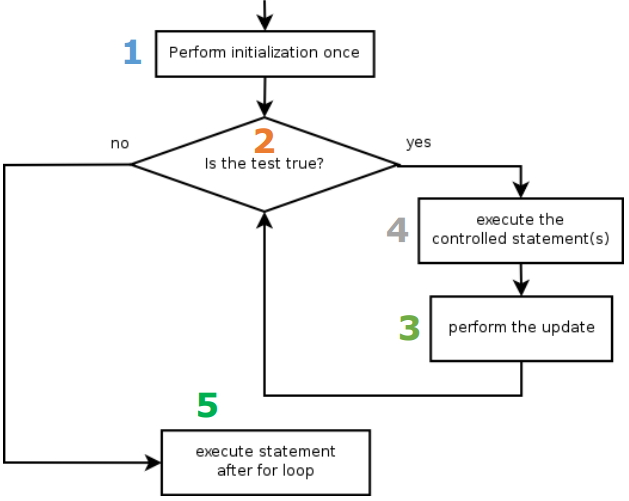
\includegraphics[scale=1]{Figures/ForLoopWalkthrough.jpg}
\end{multicols}
\item Categories of loops
  \begin{itemize}
    \item \textbf{Definite loop}: Executes a known number of times.
      \begin{itemize}
        \item The \inline{for} loops we have seen are definite loops
          \begin{itemize}
            \item Print ``Hello'' 10 times.
            \item FInd all the prime numbers up to an integer n.
            \item Print each odd number between 5 and 127
          \end{itemize}
      \end{itemize}
    \item \textbf{Indefinite loop}: One where the number of times its body repeats is not known in advance.
      \begin{itemize}
        \item Prompt the user until they type a non-negative number.
        \item Print random numbers until a prime number is printed.
        \item Repeat until the user has types ``q'' to quit.
      \end{itemize}  
  \end{itemize}
\item The {\inline{while}} loop:
  \begin{itemize}
    \item It repeatedly executes its body as long as a logical test is true.
    \item Syntax:
    \begin{lstlisting}
while (test){
    statement;
}
    \end{lstlisting}
    \item \inline{while} is better than \inline{for} because we don't know how many times we will need to increment to find the factor.
  \end{itemize}
\item Sentinel values:
  \begin{itemize}
    \item \textbf{Sentinel loop}: it repeats until a sentinel value is seen
    \item Sentinel code example:
    \begin{lstlisting}
Scanned console = new Scanner(System.in);
int sum = 0
//pull one prompt/read out of the loop
System.out.print(``Enter a number (-1 to quit): '');
int number = console.nextInt();

while (number != -1){
  sum=sum+number;    //moved to top of loop in order to avoid
                     //fencepost problems
  System.out.print(``Enter a number (-1 to quit): '');
  number = console.nextInt();
}

System.out.println(``The total is '' + sum);
    \end{lstlisting}
  \end{itemize}
\item The \inline{do/while} loop
  \begin{itemize}
    \item It performs its test at the end of each repetition.
      \begin{itemize}
        \item It guarantees that the loop's { } body will run at least once.
        \item Syntax:
\begin{lstlisting}
do{
  statement;
} while (test);
\end{lstlisting}
      \end{itemize}
  \end{itemize}
\item Arrays
  \begin{itemize}
    \item \textbf{Array}: object that stores many values of the same type.
      \begin{itemize}
        \item \textbf{element}: One value in an array.
        \item \textbf{index}: A 0-based integer to access an element from an array\\
        \\
        \begin{center}
        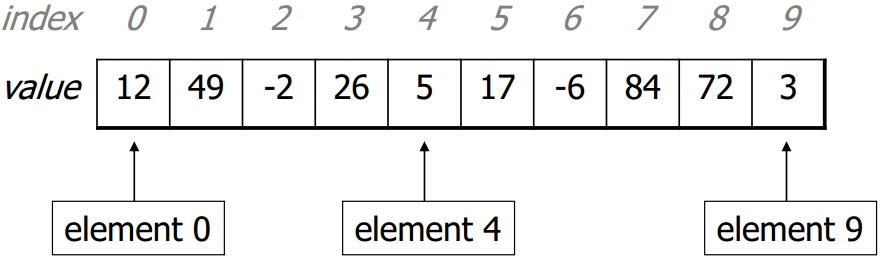
\includegraphics[scale=1]{Figures/ArrayExample.jpg}
        \end{center}
      \end{itemize}
    \item Accessing elements\\
      \begin{lstlisting}
name[index]            //access
name[index] = value;   //modify
      \end{lstlisting}
      \item One can use \inline{for} \textbf{loops} to insert elements in the array
      \item Arrays are reference types
      \item Out-of-bounds exception
        \begin{itemize}
        \item Legal indexes: between \textbf{0} and the \textbf{array's length -1}.
          \begin{itemize}
            \item Reading or writing any index outisde this range will throw an \textit{ArrayIndexOutOfBoundsException}
          \end{itemize}
        \end{itemize}
  \end{itemize}
  \item Strings
    \begin{itemize}
      \item \textbf{String}: An object storing a sequence of text characters
        \begin{itemize}
          \item Unlike most other objects, a \textit{String} is not create with \textit{new}.
          \item Syntax:
\begin{lstlisting}
String name = ``text'';
String name = expression;
\end{lstlisting} 
        \end{itemize}
    \end{itemize}
    \item Indexes
    \begin{itemize}
      \item Characters of a string are numbered with 0-based \textit{indexes}:
      \begin{itemize}
        \item First character's index: 0
        \item Last character's index: 1 less than th string's length
        \item The individual characters are values of type chars
      \end{itemize}
      \end{itemize}
      \item String methods\\
      \begin{center}
        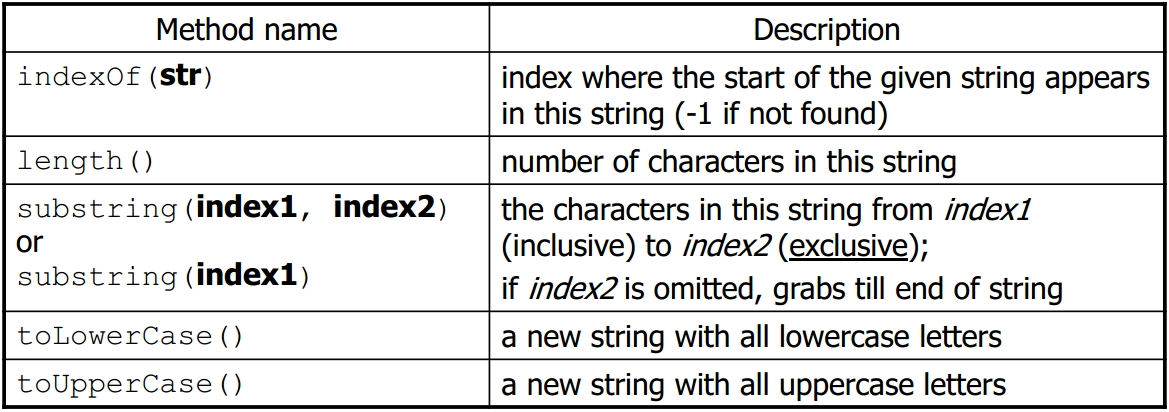
\includegraphics[scale=1]{Figures/StringMethods.jpg} 
      \end{center}
      This methods are called using the dot notation
  \item Comparing strings
    \begin{itemize}
      \item ``=='' compares objects by \textit{references}, so it often gives \textit{false} even when two \textit{Strings} have the same letters
      \item Example:\\
      \begin{center}
        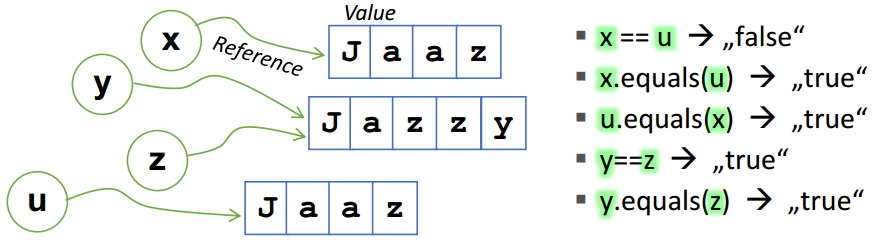
\includegraphics[scale=1.2]{Figures/StringExample.jpg}
      \end{center}
    \end{itemize}
  \item String test methods
    \begin{center}
      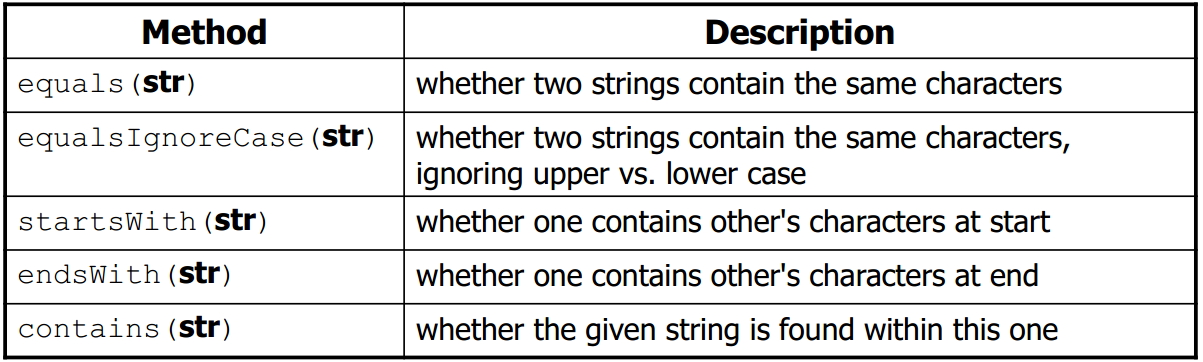
\includegraphics[scale=1]{Figures/StringTestMethods.jpg}
    \end{center}
  \begin{lstlisting}
String name = console.next ();
  if (name.startsWith(``Prof'')){
      System.out.println(``When are your office hours?'');
  } else if (name.equalsIgnoreCase(``STUART'')){
      System.out.println(``Lets talk about meta!``);
  }
  \end{lstlisting}
  \item Extract from Java API
    \begin{itemize}
      \item \inline{compareTo}
        \begin{itemize}
          \item \inline{public int compareTo(String anotherString)}\\Compares two strings lexicographically
          \item \textbf{Parameters}:\\anotherString - the String to be compared
          \item \textbf{Returns}:\\The value 0 if the argument strings is equal to this string, less tha 0 if it is lexicographically less than the string argument, value greater than 0 otherwise
        \end{itemize}
        \item \textbf{concat}
          \begin{itemize}
            \item \inline{public String concat(String str)}\\Concatenates the string argument to the end of this string.
            \item \textbf{Parameters};\\str - the String which is concatenated to the end of this String
            \item \textbf{Returns}: A string that represents the concatenation of this object's characters followed by the string argument's characters
          \end{itemize}
          \item \inline{copyValueOf}
            \begin{itemize}
              \item \inline{public static String copyValueOf(char data[])}
              \item \textbf{Parameters}:\\data - the character array
              \item \textbf{Returns}:\\A string that contains the characters of the array
            \end{itemize}
    \end{itemize}
    \item Classes and objects
      \begin{itemize}
        \item \textbf{Class}:
          \begin{itemize}
        \item A program entity that represents either:
          \begin{enumerate}
            \item A program/module, or
            \item A type of objects
          \end{enumerate}
            \item A class is a blueprint or template for constructing objects
          \end{itemize}
      \end{itemize}
     \item \textbf{Object}: An entity that combines data and behavior.
     	\begin{itemize}
     		\item \textbf{object-oriented programming (OOP)}:\\Programs that perform their behavior as interactions between objects.
     			\begin{itemize}
     				\item data: variables inside the object
     				\item behavior: methods inside the object 
     					\begin{itemize}
     						\item You interact with the methods; the data is hidden in the object
     					\end{itemize}
     				\item Constructing an object:\\\inline{Type objectName = new Type (parameters);}
     				\item Calling an object's method:\\ \inline{objectName.methodName (parameters);}
     			\end{itemize}
     	\end{itemize}
     	\item Inheritance\\
     	Eventhought there are systematic diferences, different kinds of objects often have a certain amount in common with each other.\\ Classes \textit{inherit} commonly used state and behavior from other classes, but specialized behavior and states further \todo{WTF??}
\item References and objects
	\begin{itemize}
		\item Arrays and objects use reference semantics, because of:
			\begin{itemize}
				\item \textit{efficiency}: Copying large objects slows down a program
				\item \textit{sharing}: It's useful to share an object's data among methods
				\item Example:
					\begin{lstlisting}
DrawingPanel1 panel1 = new DrawingPanel (80, 50);
DrawingPanel panel2 = panel1; //same window
panel2.setBackground(Color.CYAN);
					\end{lstlisting}
			\end{itemize}
	\end{itemize}
	\item Objects as parameters
		\begin{itemize}
			\item When an object is passed as a parameter, th object is \textit{not} copied. The parameter refers to the same object.
				\begin{itemize}
					\item If the parameter is modified, it \textit{will} affect the original object.
					\begin{lstlisting}
public static void main(String[] args) {
	DrawingPanel window = new DrawingPanel(80, 50);
	window.setBackground(Color.YELLOW);
	example(window);
}

public static void example(DrawingPanel panel) {
	panel.setBackground(Color.CYAN);
	..
}
					\end{lstlisting}
				\end{itemize}
		\end{itemize}
	\item Arrays pass by reference
		\begin{itemize}
			\item Arrays are passed as parameters by \textit{reference}.
				\begin{itemize}
					\item Changes made in the method are also seen by the caller
						\begin{lstlisting}
public static void main(String[] args) {
	int[] iq = {126, 167, 95};
	increase(iq);
	System.out.println(Arrays.toString(iq));
}
public static void increase(int[] a) {
	for (int i = 0; i < a.length; i++) {
		a[i] = a[i] * 2;
	}
}

Output:
[252, 334, 190]
						\end{lstlisting}
						 
				\end{itemize}
		\end{itemize}
	\item Arrays of objects
		\begin{itemize}
			\item \inline{null}: A value that does not refer to any object.
				\begin{itemize}
					\item The elements of an arays of objects are initialized to \inline{null}.\\
				\end{itemize}
		\end{itemize}
		\item Things you can do with null:
			\begin{itemize}
				\item store \inline{null} in a variable or an array element
				\item print a \inline{null} reference
				\item ask whether a variable or array element is \inline{null}
				\item pass \inline{null} as a parameter to a method
				\item return \inline{null} from a method (often to indicate failure)
			\end{itemize}
			\item Null pointer exception
				\begin{itemize}
					\item \textit{dereference}: To access data or methods of an object with the dot notation, such as \inline{s.length()}.
						\begin{itemize}
							\item It is illegal to dereference \inline{null} (causes an exception)
							\item \inline{null} is not any object, so it has no methods or data.
						\end{itemize}
					\item One can avoid raising an exception by simply using a if case statement before calling an object's method:
						\begin{lstlisting}
if (words[i] != null){
	...
}
					\end{lstlisting}
				\end{itemize}
	\item Encapsulation
		\begin{itemize}
			\item Encapsulation is a very important O-O concept
				\begin{itemize}
					\item Each object has 2 views. An internal view and an external view
				\end{itemize}
			\item Encapsulation is a form of protection
				\begin{itemize}
					\item Also called \textit{Information Hiding}
					\item The outside world does not have direct access to the internal implementation or representation of an object
					\item As long as the external view does not change, the internal view can take on any form without affecting the outside world
					\item Methods have the responsibility of maintaining data integritiy
				\end{itemize}
			\item Private visibility offer full encapsulation
				\begin{itemize}
					\item protected and default offer limited encapsulation
					\item public offers no encapsulation
				\end{itemize}
			\item Benefits
				\begin{itemize}
					\item Abstraction between object and clients
					\item Protects object from unwanted access
						\begin{itemize}
							\item Example: One can't fraudulently increase an \inline{Account}'s balance
						\end{itemize}
						\item Can change the class implementation later
							\begin{itemize}
								\item Example: \inline{Point} could be rewritten in polar coordinates with the same methods,
							\end{itemize}
						\item Can constrain object's state (\textbf{invariants})
							\begin{itemize}
								\item Example: Only allow \inline{Accounts} with non-negative balance.
								\item Example: Only allow \inline{Dates} with a month 1-12-
							\end{itemize}
				\end{itemize}
				\todo[inline]{Un po' ripetitivo...???}
		\end{itemize}
	\item Java access restrictions
		\begin{itemize}
			\item \textbf{Packages}: defin a name space
			\item Default package used in the absence of a package declaration
			\item For class members you can specify which other objects can access (read/write or invoke) them
				\begin{itemize}
					\item (default)[nothing]: accessible in current package
					\item \inline{public}: everywhere
					\item \inline{private}: only from this class
					\item \inline{protected}: accessible in current package and all subclasses, regardless of their package
				\end{itemize}
		\end{itemize}
	 \item Private fields
	 	\begin{itemize}
	 		\item A field that cannot be accessed from outside the classe\\
	 		\inline{private type name;}
	 	\end{itemize}
	 \item The \inline{this} keyword
	 	\begin{itemize}
	 		\item \inline{this}: Refers to the implicit parameter inside your class.\\\textit{(a variable that stores the object a method is called)}
	 			\begin{itemize}
	 				\item Refer to a field \inline{this.field}
	 				\item Call a method: \inline{this.method(parameters);}
	 				\item One constructor can call another: \inline{this(parameters);}
	 			\end{itemize}
	 	\end{itemize}
	 \item Class versus Instance Methods
	 	\begin{itemize}
	 		\item \textbf{Class methods} are marked by the \inline{static} keyword.
	 			\begin{itemize}
	 		\item They are not called via an object reference but directly via the class
	 		\item Can be called from a static context.
	 		\item often serve as utility function.
	 		\item They are generic and need no access to object variables and methods
	 			\begin{lstlisting}
classDatum {
	privateintday, month, year;
	staticString monthName(Datum d)
		{
			if(d.month== 1) return "January";
			if... 			return "February";
			...
		}
	...
}
	 			\end{lstlisting}
	 			\end{itemize}
	 	\end{itemize}
\end{itemize}
\section{Threads}
	\begin{itemize}
		\item Multitasking
			\begin{itemize}
				\item Concurrent execution of multiple tasks
				\item Time multiplexing of CPU
					\begin{itemize}
						\item Creates impression of parallelism, even on single core/CPU system
					\end{itemize}
				\item Allows for asynchronous I/O
					\begin{itemize}
						\item I/O devices and CPU are truly parallel
						\item 10ms waitinf for HDD allows other proceses to execute $>10^{10}$ instructions
					\end{itemize}
			\end{itemize}
		\item Process ontext
			\begin{itemize}
				\item Multiple concurrent instances of \textbf{same program} (e.g., mutiple browser windows)
				\item Multiple applications (=processes) in parallel
				\item Each process has a \textbf{context}
					\begin{itemize}
						\item Instruction counter
						\item Register content
						\item Variable vaues
						\item Stack content
						\item Resourcing (device access, open files)
					\end{itemize}
			\end{itemize}
		\item Process States\\
		\begin{center}
		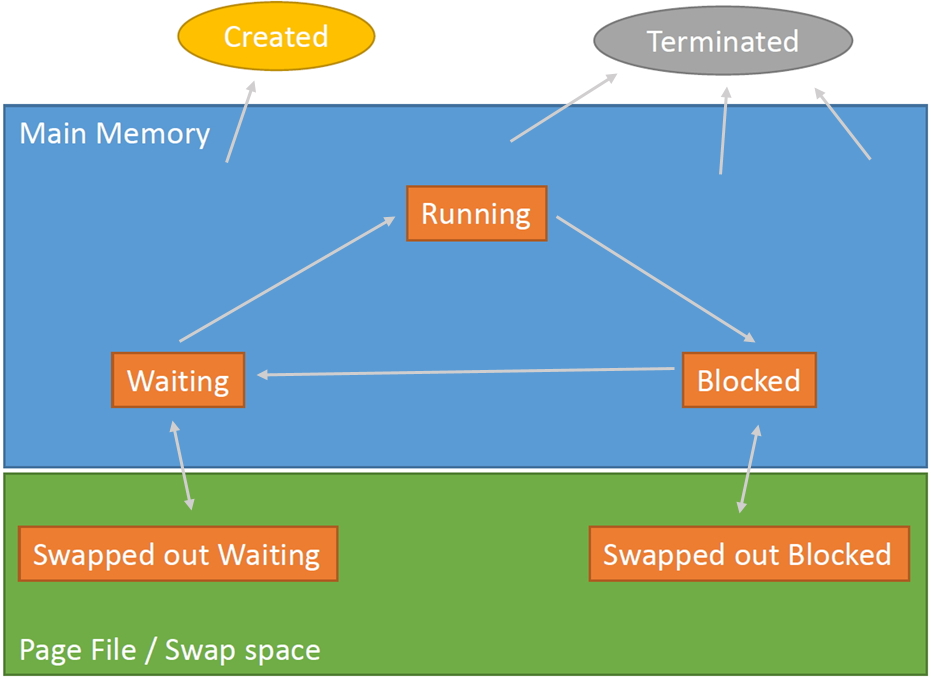
\includegraphics[scale=1]{Figures/ProcessState2.jpg}
		\end{center}
		\item Process management
			\begin{itemize}
				\item Proceses need resources
					\begin{itemize}
						\item CPU time, Memory, etc.
					\end{itemize}
				\item OS manages processes:
					\begin{itemize}
						\item Starts processes
						\item Terminates processes (frees resources)
						\item Controls resource usage (prevents monopolizing CPU tim)
						\item Schedules CPU time
						\item Synchronizes processes if necessary
						\item Allows for inter process communication
					\end{itemize}
			\end{itemize}
		\item Process control blocks (PCB)\\
		\begin{center}
			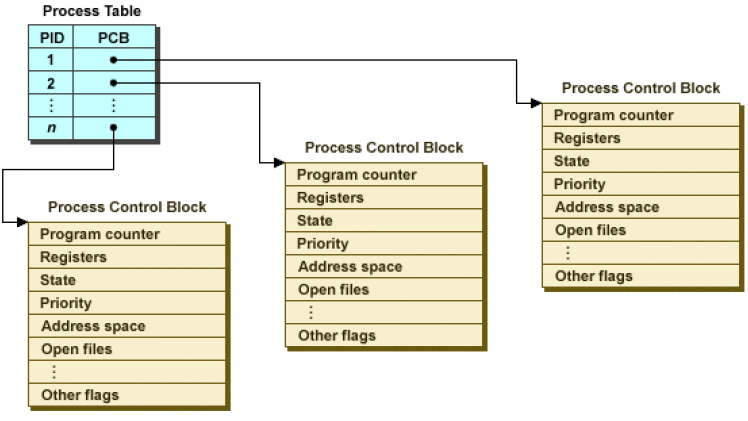
\includegraphics[scale=1.5]{Figures/PCB.jpg}
		\end{center}
\end{itemize}
\subsection*{Java Threads}
	\begin{itemize}
		\item Threads (light weight processes)
			\begin{itemize}
				\item \textbf{Threads} (of control) are independent sequences of execution, but multiple threads \textbf{share the same address space}
					\begin{itemize}
						\item Threads are not shielded from eachother
						\item Threads share resources and can communicate moer easily
					\end{itemize}
				\item Context switching between threads is much more efficient for threads
					\begin{itemize}
						\item No change of address space
						\item No autmoatic scheduling
						\item No saving / (re-)loading of PCB state
					\end{itemize}
				\item Many more thread changes possible than process switches per unit of time
			\end{itemize}
		\item Advantages of MUltithreading
			\begin{itemize}
				\item Reactive systems-constantly monitoring
				\item More responsive to user input-GUI application can interrupt a time-consuming task
				\item Server can handle multiple clients simultaneously
				\item Can take advantage of parallel processing
			\end{itemize}
		\item Multithreading conceptually\\
			\begin{center}
				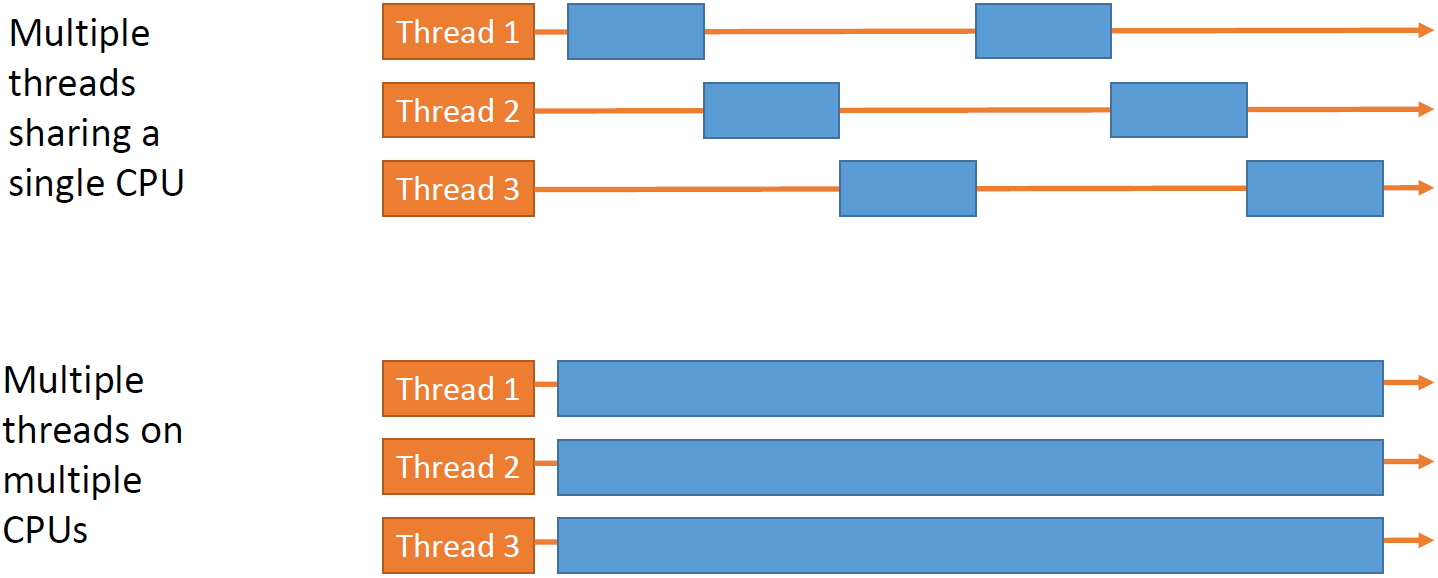
\includegraphics[scale=1]{Figures/MultithreadingConceptually.jpg}
			\end{center}
		\item Two options to create Java Threads
			\begin{itemize}
				\item Extend \inline{java.lang.Thread} class
					\begin{itemize}
						\item Override run method (must be overridden
						\item run() is called when execution of the thread begins
						\item A thread terminates when run() returns
						\item start() method invokes run()
						\item Calling run() does not create a new thread
					\end{itemize}
				\item Implement \inline{java.an.Runnable} thread
					\begin{itemize}
						\item If already intheriting another class (i.e., JApplet)
						\item Single method: public vodi rn()
						\item Thread classh implements Runnable
					\end{itemize}
			\end{itemize}

	\end{itemize}


%=============== START OF MIDTERM 2, NEEDS REVISION ================
\setcounter{section}{10}%required to start at chapter 11
\section{Synchronization: Beyond Locks}
\begin{itemize}
\item Locks provide means to enforce atomicity via mutual exclusion 
\item They lack means for threads to communicate about changes, e.g. changes in state
\item Example: producer/consumer (p/c) queues (think: bakery)
\begin{itemize}
\item can be used for data-flow parallel programs, e.g. pipelines where a mean to transfer X from the producer to the consumer is needed
\item There might be multiple producers or (not xor) multiple consumers
\item For an implementation a circular buffer (with a fixed size) can be used with simple \textbf{dequeue()}/\textbf{enqueue()} and an “in” and “out” counter. Both functions use a shared (reentrant) lock and rely on helper functions to check for full/empty queue\footnote{Note: If you have a try-catch-finally block and there is a return statement (assume it will be called no matter what) in the ``try'' part and an unlock() in the ``finally'' part, the finally part will always be executed (and thus also the lock released!).}
\item If you use a busy wait (while loop) there is a chance of a deadlock (and CPU running high). Using sleep for synchronization as another approach is generally discouraged
\item The solution is a condition variable which (ideally) notifies the threads upon change
\end{itemize}
\item A condition interface provides the following methods:
\begin{itemize}
\item \inline{await()}: the current thread waits until it is signaled. 
\begin{itemize}
\item Called with the lock held
\item Releases the lock atomically and waits for thread to be signaled
\item When returns, it is guaranteed to hold the lock
\item Thread always needs to check condition
\end{itemize}
\item \inline{signal()}: wakes up one waiting thread. Called with the lock held
\item \inline{signalAll()}: wakes up all waiting threads. Is called with the lock held
\end{itemize}
\textbf{\underline{Conditions are always associated with a lock}}
\item Check then act! 
\item Conditions can also be used with intrinsic locks where each object can act as a condition, implementing \inline{.notify()}, \inline{.notifyAll()}, .\inline{wait()}. 
\begin{itemize}
\item They do not allow for multiple conditions (e.g. different condition for Full/Empty in P/C queues)
\end{itemize}
\item \inline{Object.wait} and \inline{Condition.await}: 
\begin{itemize}
\item always have a condition predicate
\item always test the condition predicate: before calling wait and after returning from wait 
\item always call wait in a loop
\item Ensure state is protected by lock associated with condition
\end{itemize}
\item Semaphores\footnote{Language background: semaphore is fancy for traffic light in English (see also Spanish).} 
\begin{itemize}
\item Invented by Dijkstra
\item Operations:
\begin{itemize}
\item \textbf{Initialize} to an integer value
\begin{itemize}
\item After initialization only wait/signal operations are allowed
\end{itemize}
\item \textbf{Acquire}:
\begin{itemize}
\item Integer value is decreased by one
\item If $<0\to$ thread suspends execution
\end{itemize}
\item \textbf{release}
\begin{itemize}
\item Integer value is decreased by one
\item If there is at least a thread waiting, one of the waiting threads resumes execution
\end{itemize}
\end{itemize}
\item Notes on Semaphores:
\begin{itemize}
\item A thread cannot know the value of a semaphore, and thus cannot know whether its execution will be suspended if it calls \inline{acquire()}
\item There is no rule about what thread will continue its operation after \inline{release()}
\item Operations are traditionally also referred to as
\begin{itemize}
\item \textsl{P()}: acquire (also wait)
\item \textsl{V()}: release (also signal)
\end{itemize}
\end{itemize}
\item Building a lock with a semaphore:
\begin{itemize}
\item mutex\footnote{Mutual Exclusion Locks: make sure that at most one thread owns the lock} = Semaphore(1); Initialize mutex using a semaphore, and set it to unlocked (1)
\item lock mutex $\to$ mutex.acquire(); only one thread is allowed into the critical section
\item unlock mutex $\to$ mutex.release(); One other thread will be woken up
\item Semaphore number:
\begin{itemize}
\item $1=$ unlocked
\item $0=$ locked
\item $-x=$ locked and $x$ threads are waiting to enter
\end{itemize}
\end{itemize}
\item You can (of course) also use semaphore for p/c queues, however you need to use two semaphores to order the operations (and to prevent a deadlock).
\end{itemize}

\item Barriers
\begin{itemize}
\item Rendezvous for arbitrary number of threads i.e. every thread has to wait up for all other threads to arrive at a certain point
\item Can be implemented for $n$ threads with:
\begin{itemize}
\item  two semaphores (and one count variable): 
\begin{itemize}
\item One as a mutex (used to atomically increment the counter) with default = 1 
\item One as a barrier with default = 0 (which is released if count $== n$ and otherwise only acts as acquire-and-release-immediately).
\end{itemize}

\begin{lstlisting}
count = 0
mutex = Semaphore(1)
barrier = Semaphore(0)

mutex.acquire()
   count = count + 1
mutex.release()

if (count == N){
   barrier.release()
}

barrier.acquire()
barrier.release()
\end{lstlisting}
\end{itemize}
\item If you want a reusable barrier for n threads (aka 2-phase barrier) with semaphores, you need a count, a mutex and two barriers for it to be thread-safe.
\begin{lstlisting}
count=0; mutex = Semaphore(1); bar0 = Semaphore(0); bar1 = Semaphore(1);

mutex.acquire()
count +=1
if (count == N){
  bar1.acquire()
  bar0.release()
}
mutex.release()

bar0.acquire()
bar0.release()

mutex.acquire()
count -= 1
if (count == 0){
  bar0.acquire()
  bar1.release()
}
mutex.release()

bar1.acquire()
bar1.release()
\end{lstlisting}

\end{itemize}


\end{itemize}

\section{Advanced (and other) Topics}
\begin{itemize}
\item Locks can be implemented with low-level atomic operations (basic operations that are guaranteed to be atomic) and busy wait loops (a thread continuously checks a condition)
\begin{itemize}
\item Example: Peterson Lock
\begin{lstlisting}
AtomicBoolean t0 = new AtomicBoolean(false);
AtomicBoolean t1 = new AtomicBoolean(false);
AtomicInteger victim = new AtomicInteger(0);
lock:
    my_t.set(true)
    victim.set(me);
    while (other_t.get() == true &&victim.get() == me)
        ;
	
	unlock:
        my_t.set(false);
\end{lstlisting}
Two AtomicBooleans (one per thread) and an AtomicInteger which decides which thread will be selected.
\end{itemize}
\item In order to make our life easier, we need rich(er) atomic operations for AtomicInteger: 
\begin{itemize}
\item \inline{getAndSet(val)} (atomically { set to val, return old value })
\item \inline{getAndAdd(val)}
\item \inline{getAndIncrement}
\item \inline{getAndDecrement}
\item \inline{CompareAndSet} (CAS for short)
\end{itemize}
\item Lock using \inline{getAndSet}: mutex is an AtomicBoolean which is set to either true or false on lock or unlock (resp.)
\begin{lstlisting}
mutex = new AtomicBoolean(false);
lock:
  while (mutex.getAndSet(true));
unlock:
  mutex.set(false);
\end{lstlisting}
\item CAS; performs atomically the following (optimistically): 
\begin{lstlisting}
atomic_int.compareAndSet(int old, int new)

atomically {
  if (current_val == old) {
    current_val=new
    return true
  }
  else {
     return false
  }
}
\end{lstlisting}
\item Lock using \inline{getAndSet}: 
\begin{lstlisting}
mutex = new AtomicBoolean(false);

lock:
  while (mutex.getAndSet(true));

unlock:
  mutex.set(false);
\end{lstlisting}
\item Busy-wait
\begin{itemize}
\item Check continuously for a value
\item Wastes CPU-time 
\item Alternative: exponential backoff
\item Ideally we would like some sort of notification mechanism
\end{itemize}
\item Mutexes: 
\begin{itemize}
\item Locks that suspend the execution of threads while they wait are typically called mutexes (vs spinlocks)
\item Scheduler (typically from the OS) support is required
\item They do not waste CPU time but they have higher wakeup latency
\item Hybrid approach: spin and then sleep
\end{itemize}
\item Locks performance: 
\begin{itemize}
\item Uncontended case: 
\begin{itemize}
\item When threads do not compete for the lock
\item Lock implementations try to have minimal overhead, typically just the cost of an atomic operation
\end{itemize}
\item Contended case: 
\begin{itemize}
\item When threads do compete for the lock
\item Can lead to significant performance degradation, as well as starvation
\end{itemize}
\end{itemize}
\item Disadvantages of locking
\begin{itemize}
\item locks are pessimistic by design, they assume the worse/worst and enforce mutual exclusion
\item Performance issues: 
\begin{itemize}
\item Overhead for each lock taken even in uncontended case
\item Contended case leads to significant performance degradation
\end{itemize}
\item blocking semantics (wait until acquire lock)
\begin{itemize}
\item  if a thread is delayed for a reason (e.g., scheduler) when in a critical section $\rightarrow$ all threads suffer
\item Leads to deadlocks (and also livelocks)
\end{itemize}
\end{itemize}
\item Non-blocking algorithms: 
\begin{itemize}
\item Locks: a thread can indefinitely delay another thread
\item Non-blocking: failure or suspension of one thread cannot cause failure or suspension of another thread
\item Lock-free: at each step, some thread can make progress 
\item Typically built using CAS operations(more powerful than plain-atomic)
\begin{itemize}
\item see lecture slides for stack example (Page 18)
\item Non-blocking counter example:
\begin{lstlisting}
public class CasCounter {
  private AtomicInteger value;

  public int getVal() {
    return value.get();
  }

  public int inc() {
    int v;
    do {
       v = value.get();
    } while (!value.compareAndSet(v, v+1));
    return v+1;
  }
}
\end{lstlisting}
\end{itemize}
\end{itemize}
\end{itemize}

\subsection{An overview of java.util.concurrent}
\begin{itemize}
\item Lock interface:
\begin{lstlisting}
void lock()
void lockInterruptibly()

boolean tryLock()
boolean tryLock(long time, TimeUnit unit)

void unlock()
Condition newCondition()
\end{lstlisting}
Interface implemented by ReentrantLock


\item Readers-Writer Lock
\begin{itemize}
\item Observation: multiple readers can concurrently access state
\item Different roles:
\begin{itemize}
\item Readers: Allow to co-exist with other readers
\item Writers: Exclusive access
\end{itemize}
\item Beneficial for ``read-mostly'' workloads
\item Can be implemented with semaphores but fairness might be an issue leading to starvation\footnote{Starvation: when a particular thread cannot resume execution; different from deadlock, where all the threads are unable to proceed}  unless prevented by means to notify the read lock about waiting writers
\end{itemize} 
\item Java collections
\begin{itemize}
\item Aggregate Objects: Objects that group multiple elements into a single unit
\item Interfaces (e.g. Collection, List, Set, SortedSet,\dots)
\item Implementations (e.g. ArrayList and LinkedList for List)
\item Algorithms (e.g. Sort)
\end{itemize}
$\to$ Based on Java Generics
\item Synchronized Collections: 
\begin{itemize}
\item Vector, HashTable (JDK 1.0)
\item java.util.collections (JDK 1.2):
\begin{itemize}
\item synchronizedList(List$<$T$>$ list)
\item synchronizedMap(Map$<$K,V$>$ m)
\item synchronizedSet(Set$<$T$>$ s)
\item synchronizedSortedMap(SortedMap$<$K,V$>$ m)
\item synchronizedCollection(Collection$<$T$>$ c)
\end{itemize}
\item They are synchronized wrapper classes
\item Wrap every public method in a synchronized block
\item Thread-safe
\item Client-side locking for compound actions (e.g. iteration, put-if-absent)
\item Poor concurrency: single, collection-wide lock
\end{itemize}
\item Concurrent Collections: 
\begin{itemize}
\item Thread-safe
\item Not governed by a single lock
\begin{itemize}
\item Cannot be locked for exclusive access
\item No client-side locking
\item Common compound operations added (e.g. put-if-absent, replace-if-equal,\dots)
\end{itemize}
\item Examples:
\begin{itemize}
\item ConcurrentHashMap 
\begin{itemize}
\item As a replacement for synchronized hash-based map
\end{itemize}
\item ConcurrentSkipListMap, ConcurrentSkipListSet
\begin{itemize}
\item As a replacement for synchronized tree-based impls.
\end{itemize}
\item CopyOnWriteArrayList, CopyOnWriteArrayList
\begin{itemize}
\item Frequent reads, infrequent writes
\end{itemize}
\end{itemize}
\end{itemize}
\item Queues: 
\begin{itemize}
\item BlockingQueue
\begin{itemize}
\item ArrayBlockingQueue, LinkedBlockingQueue (FIFO)
\item PriorityBlockingQueue (ordered)
\end{itemize}
\item TransferQueue: allows to wait until a consumer receives item; 
\item SynchronousQueue: hand-of, no internal capacity 
\item Dequeue/BlockingDeque: 
\begin{itemize}
\item Allows efficient removal/insertion at both ends (head/tail)
\item Work stealing pattern
\end{itemize}
\end{itemize}
\item Synchronizers: 
\begin{itemize}
\item Semaphores
\item CyclicBarrier (Java's barrier)
\item CountDownLatch (thread wait until countdown reaches zero)
\begin{itemize}
\item \inline{CountDownLatch(int count)} - initialize latch
\item \inline{.await()} - wait for event
\item \inline{.countDown()} - decrement count
\end{itemize}
\end{itemize}
\item Future: \\
interface Future$<$V$>$
\begin{itemize}
\item Represents a result (type T) for an asynchronous computation
\item \inline{.get()} - wait for result
\item \inline{.isDone()} - check if task is completed
\item \inline{.cancel()} - attempt to cancel computation
\end{itemize}
\end{itemize}

%%%% FROM HERE!
\section{Parallel Tasks}
Example for most of this section: $\sum x_i$
\begin{lstlisting}
public static int sum(int[] xs) {
	int sum = 0;
	for (int x: xs)
		sum += x;
 	return sum;
}
\end{lstlisting}
\begin{itemize}
\item When writing a parallel program, write a sequential version first! This is useful for knowing the results are correct and evaluate the performance of the parallel program
\item Divide-and-conquer approach: recursive sum with the lower and upper half of the remaining part which cuts off at size = 1 is a lot slower $(\times 10)$. 
\item Task parallel model, basic operations: 
\begin{itemize}
\item create a parallel task and wait for the parallel tasks to complete
\item  when using D\&C a task for the first and second part (one each) are created, and upon finishing the operations, their results are combined
\end{itemize}
\item One thread per task: expensive to create, consumes many resources and is scheduled by the OS - generally inefficient
\begin{itemize}
\item In General: using one thread per task is highly inefficient 
\end{itemize}
\item ExecutorService: A (huge) amount of tasks is handled by an interface which assigns a thread from a thread pool to each task and returns a Future
\item Note: Runnable doesn’t return a result, Callable does
\item ExecutorService and recursive sum\footnote{Have a look at the code in the slides, pp36-38} : task is described as the array to be summed and the region for which the task is responsible for, additionally an instance to the ExecutorService is passed so that the task can spawn other tasks; problems (observation: no result returned): Tasks create other tasks and then wait for results, when they are waiting they are keeping threads busy, other tasks need to run so that the recursion reaches its bottom, system does not know that tasks waiting need to be removed so that other tasks can run due to: tasks create other tasks (which is not supported) and work partitioning (splitting up work) is part of the task - we can decouple work partitioning from solving the problem
\item Fork/Join framework with ForkJoinTask 
\begin{itemize}
\item \inline{fork()} creates a new task
\item \inline{join()} returns the result when task is done
\item \inline{invoke()} executes task without creating a new task
\item subclasses need to define \inline{compute()}
\end{itemize}
implements Future and ForkJoinPool implements ExecutorService. Note \inline{fork()}, , \inline{join()}, \inline{join()} doesn’t work (well) in Java, solved by using\footnote{``+'' is in this case the arithmetic addition but can also be something else of a combining nature}
\begin{lstlisting}
t1.fork(), r2 = t2.compute()
return r2 + t1.join()
\end{lstlisting}
\item Problems of overhead: bad speedup due to too much overhead (scheduling etc.), can be solved by making each task work more, here: increase cutoff
\end{itemize}

\section{Transactional Memory (TM)}
\begin{itemize}
\item Aims at removing the burden of having to deal with locks from the programmer and place it on the system instead
\item Problems with locks: 
\begin{itemize}
\item ensuring ordering and correctness is really hard and locks are not composable
\item locks are pessimistic, performance overhead
\item locking mechanism is hard-wired to the program (separation not possible and change of synchronization scheme results in changing all of the program)
\end{itemize}
\item With TM, the programmer explicitly defines atomic code sections and is only concerned with the \textsl{what} and not the \textsl{how} (declarative approach)
\item TM benefits: 
\begin{itemize}
\item easier, less error-prone, higher semantics, composable, optimistic by design
\item changes made by a transaction are made visible atomically
\item  transactions run in isolation - while a transaction is running, effects from other transactions are not observed (as if transaction takes a snapshot of the global state when it begins and operates on that snapshot)
\item Note: while locks enforce atomicity via mutual exclusion, transaction does not require that
\end{itemize}
\item TM is inspired by transactions in databases where transactions are vital 
\begin{itemize}
\item ACID: \textbf{A}tomicity, \textbf{C}onsistency, \textbf{I}solation, \textbf{D}urability
\end{itemize}
\item Implementation of TM:
\begin{itemize}
\item Keep track of operations performed by each transaction
\item Concurrency control, system ensures atomicity and isolation properties
\end{itemize}
\item Transactions can be aborted if a conflict has been detected by the concurrency control (CC) mechanism 
\begin{itemize}
\item aborts are possible e.g. if there’s a deadlock
\item on abort, a transaction can be retried automatically or the user is notified
\end{itemize}
\item Where TM is/can be implemented: 
\begin{itemize}
\item Hardware TM : can be fast but cannot handle big transactions
\item Software TM (STM) : in the language, greater flexibility, performance might be challenging
\item Hybrid TM; TM is still work in progress with many different approaches and is still under active development
\end{itemize}
\item Design choice: 
\begin{itemize}
\item strong vs weak isolation:
\begin{enumerate}
\item[Q.] What happens when shared state accessed by a transaction, is also accessed outside of a transaction? Are the transactional guarantees still maintained? 
\item[A.]
\begin{itemize}
\item Strong isolation: Yes, 
\begin{itemize}
\item easier for porting existing code
\item difficult to implement, overhea
\end{itemize}
\item Weak isolation: No
\end{itemize}
\end{enumerate}
\item Nesting:
\begin{enumerate}
\item[Q.] What are the semantics of nested transactions? (Note: nested transactions are important for composability)
\item[A.]
\begin{itemize}
\item flat nesting (inner aborts $\rightarrow$ outer aborts)
\item inner commits $\rightarrow$ changes visibly only if outer commits, closed nesting (inner abort does not result in an abort for the outer transaction
\item inner transaction commits $\rightarrow$ changes visible to outer transaction but not to other transaction
\item only when outer transaction commits, changes of inner transactions become visible), other approaches (e.g. open nesting)
\end{itemize}
\end{enumerate}
\end{itemize}
\item The more variables are part of a transaction (and thus protected) the easier it gets to port existing code but the more difficult to implement ,too (need to check every memory operation)
\item Reference-based STMs: mutable state is put into special variables
\begin{itemize}
\item  these variables can only be modified inside a transaction, everything else is immutable (or not shared; see functional programming)
\end{itemize}
\item Mechanism of retry: 
\begin{itemize}
\item implementations need to track what reads/writes a transaction performed to detect conflicts, typically called read-/write-set of a transaction
\item when retry is called, transaction aborts and will be retried when any of the variables that were read, change
\end{itemize}
\item Issues with transactions:
\begin{itemize}
\item it is not clear what the best semantics for transactions are
\item getting good performance can be challenging
\item I/O operations: can we perform I/O operations in a transaction?
\end{itemize}
\item I/O  in transactions: in general, I/O operations cannot be rolled-back and thus generally cannot be aborted
\begin{itemize}
\item that is why I/O operations are not allowed in transactions
\item one of the big issues with using TM
\item (some) STMs allow registering I/O operations to be performed when the transaction is committed
\end{itemize}
\end{itemize}

\section{Designing Parallel Algorithms}
\begin{itemize}
\item There are no rules whatsoever, yet - as (very) often - it is a matter of experience
\item The following points can/should be considered:
\begin{itemize}
\item Where do the basic units of computation (tasks) come from? 
\begin{itemize}
\item This is sometimes called ``partitioning'' or ``decomposition''
\item Depending on the problem partitioning in terms of input and/or output can make sense or functional decomposition might yield better results
\end{itemize}
\item How do the tasks interact? 
\begin{itemize}
\item We have to consider the dependencies between tasks (dependency, interaction graphs)
\item Dependencies will be expressed in implementations as communication, synchronization and sharing (depending upon the machine model)
\end{itemize}
\item Are the natural tasks of a suitable granularity? 
\begin{itemize}
\item Depending upon the machine, too many small tasks may incur high overheads in their interaction. Should they be collected together into super-tasks?
\end{itemize}
\item How should we assign tasks to processors? 
\begin{itemize}
\item In the presence of more tasks than processors, this is related to scaling down
\item The``owner compute'' rule is natural for some algorithms which have been devised with a data-oriented partitioning
\item We need to ensure that tasks which interact can do so as (quickly) as possible.
\end{itemize}
\end{itemize}
\item D\&C is a very important technique and particularly helpful in PP since the recursive step can instead be parallelized
\item Number of threads to be used: 
\begin{itemize}
\item ``Runtime.getRuntime().availableProcessors()'' might be the right amount but your program may not get access to all cores
\item too few threads are bad because core(s) is/are idle
\item too many threads can be bad because of the overhead\footnote{This depends on the actual overhead the language introduces (in Java rather big)}
\end{itemize}
\item Sorting : If the array is sorted the following condition must hold (equal only if $A_i=A_j$): 
\begin{itemize}
\item $A_i\leq A_j$  for $i<j$
\item features of a sorting algorithm:
\begin{itemize}
\item stable (duplicate data is allowed and the algorithm does not change duplicate's original ordering relative to each other), in-place ($\mathcal{O}(1)$ auxiliary space), non-comparison
\item horrible $\Omega(n^2 )$: bogo, stooge
\item simple $\mathcal{O}(n^2 )$: insertion\footnote{At step $k$, put the $k^{th}$ input element in the correct position among the first elements} , selection\footnote{At step $k$, find the smallest element among the unsorted elements and put it at position $k$} , bubble, shell
\item fancier $\mathcal{O}(n \log⁡ n )$: heap, merge, quick sort (on average!)
\item specialized $\mathcal{O}(n)$: bubble, radix
\end{itemize}
\end{itemize}
\item Linked Lists and Big Data: 
\begin{itemize}
\item Mergesort can very nicely work directly on linked lists
\item Heapsort and Quicksort do not;
\item InsertionSort and SelectionSort can too but slower
\item Mergesort also the sort of choice for external sorting
\end{itemize}
\item Differences: 
\begin{itemize}
\item Quicksort and Heapsort jump all over the array
\item Mergesort scans linearly through arrays
\item In-memory sorting of blocks can be combined with larger sorts
\item Mergesort can leverage multiple disks
\end{itemize}
\item PRAM model: 
\begin{itemize}
\item processors working in parallel, each is trying to access memory values
\item when designing algorithms, the type of memory access required needs to be considered
\item scheme for naming different types: [concurrent $\mid$ exclusive]READ[concurrent $\mid$ exclusive]WRITE\footnote{Abbreviated as E/C and R/W; ERCW is never considered }
\item typically CR are not a problem since the memory isn’t changed whereas EW requires code to ensure writing is exclusive
\item PRAM is helpful to envision how it works and the needed data access pattern but isn’t necessarily the way processors are arranged in practice
\end{itemize}
\end{itemize}

\section{Java GUIs - MVC - Parallelism}
\todo[inline]{Don’t get me wrong, but I’m having a hard time writing up this lecture…}
\begin{itemize}
\item (important) concepts: 
\begin{itemize}
 \item MVC (model (application domain, state and behavior)
\item view (display layout and interaction views)
\item controller (user input, device interaction))
\item layout managers
\item event-driven design  (listener, worker\footnote{In Swing, this implements Runnable} , callback, fire/handle)
\item GUI (painting)
\end{itemize}
\item Swing threads: 
\begin{itemize}
\item initial\footnote{Main thread}
\item event dispatch\footnote{Drawing/painting the GUI}
\item worker thread\footnote{Background thread, can be used for (heavy) computation to keep GUI responsive}
\end{itemize}
\item MVC: 
\begin{itemize}
\item Model: complete, self-contained representation of object managed by the application, provides a number of services to manipulate the data, computation and persistence issues
\item View: tracks what is needed for a particular perspective of the data, presentation issues
\item Controller: gets input from the user, and uses appropriate information from the view to modify the model, interaction issues
\end{itemize}
\end{itemize}

\section{Concurrent Message Passing}
\begin{itemize}
\item Goal: avoid (mutable) data sharing, instead use concurrent message passing (actor programming model) since many of the PP problems (so far) are due to shared state
\item isolated mutable state: 
\begin{itemize}
\item state is mutable, but not shared
\item each thread/task has its private state
\item tasks cooperate with message passing
\end{itemize}
 \begin{figure}[ht]
\centering
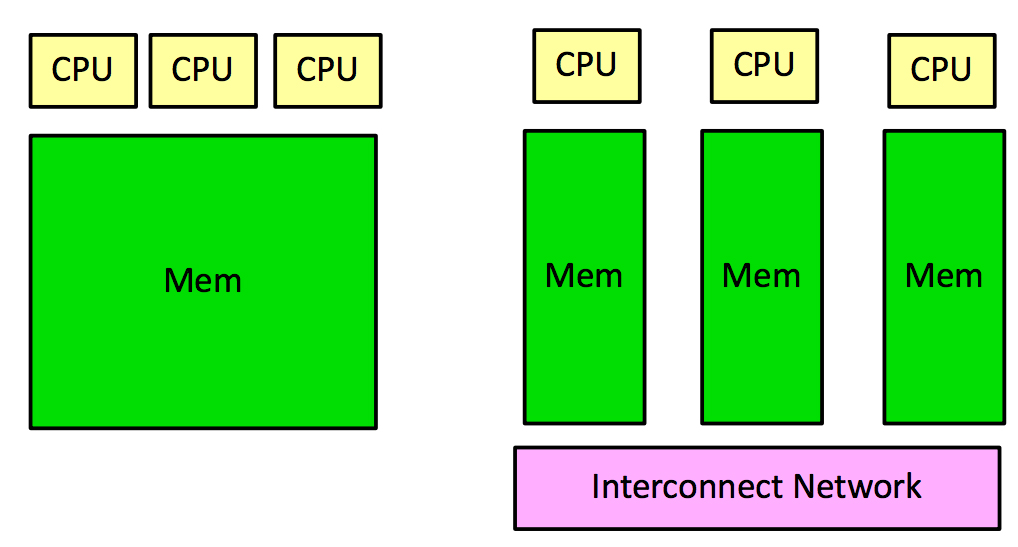
\includegraphics[width=85mm]{Figures/image1.jpg}
\end{figure}

\item shared memory architecture (left side in image)
\begin{itemize}
\item message passing and sharing state is used
\item message passing can be slower than sharing data yet is easier to implement and to reason about 
\end{itemize}
\item Distributed Memory Architecture (right side in image)
\begin{itemize}
\item sharing state is challenging and often inefficient, using almost exclusively message passing
\item additional concerns such as failures
\end{itemize}
\item Message passing works in both shared and distributed memory architectures making it more universal
\begin{itemize}
\item Example: shared state counting (i.e. atomic counter) with increase() and get(): 
\begin{enumerate}
\item[\#1:] one counter thread, the other threads ask for its value
\item[\#2:] every thread has its own (local) counter (Java: ThreadLocal), when sum is requested all threads return the value of their local counter
\end{enumerate}
\item Example: bank account: 
\begin{itemize}
\item sequential programing: single balance
\item PP shared state: single balance \& protection
\item PP distributed state: each thread has a local balance (budget), threads share balance coarsely 
\end{itemize}
\end{itemize}
\item distributed bank account (cont.): each task can operate independently, only communicate when needed
\item Synchronous vs. Asynchronous messages: 
\begin{itemize}
\item sync: send blocks until message is received (Java: SynchronousQueue)
\item async: send does not block ("fire-and-forget"), placed into a buffer for receiver to get (Java: BlockingQueue, async as long as there is enough space (to prevent memory overflow))
\end{itemize}
\item concurrent message passing programming models: 
\begin{itemize}
\item actors: state-full tasks communicating via messages (e.g. erlang)
\item channels\footnote{not an official term}: can be seen as a level of indirection over actors, Communicating Sequential Process (CSP) (e.g. go)
\end{itemize}
\item go (by Google): language support for: lightweight tasks (aka goroutines), typed channels for task communications which are synchronous (unbuffered) by default 
\item actor programming model: 
\begin{itemize}
\item a program is a set of actors that exchange (async) messages
\item actor embodies:
\begin{itemize}
\item state
\item communication
\item processing
\end{itemize}
\item An Actor may:
\begin{itemize}
\item process messages
\item send messages
\item change local state
\item create new actors
\end{itemize}
\end{itemize}
\item event-driven programming model: a program is written as a set of handlers (typical application: GUI)
\item Erlang: 
\begin{itemize}
\item functional language
\item developed for fault-tolerant applications, if no state is shared, recovering form errors becomes much easier
\item concurrent, following the actor model
\item open-source 
\end{itemize}
\item Actor examples: 
\begin{itemize}
\item Distributor: forward received messages to a set of names in a round-robin fashion
\begin{itemize}
\item State: an array of actors with the array index of the next actor to forward a message
\item Receive: messages $\rightarrow$ forward message and increase index (mod), control commands (e.g. add/remove actors)
\end{itemize}
\item Serializer: unordered input (e.g. due to different computation speed) $\rightarrow$ ordered output; 
\begin{itemize}
\item State: sorted list of received items, last item sent
\item Receive: if we receive an item that is larger than the last item plus one, add it to the sorted list; if we receive an item that is equal to the past item plus one: send the received item plus all consecutive items form the last and reset the last item
\end{itemize}
\end{itemize}
\item concurrent message passing in Java: 
\begin{itemize}
\item For simple applications, queues can be used which might be difficult especially for large tasks
\item Instead use Akka framework (written in Scala, interface for Java): follows the actor model (async messages), rich set of features\footnote{important methods to be overridden: preStart(), onReceive()} 
\end{itemize}

\item Akka actors example: 
\begin{itemize}
\item ping-pong: client sends $n$ PINGs to server which responds with Pong upon receiving back to sender, master stops execution when receiving DONE
\item Version 2 with restart on DONE: add a message type SETUP to the client passing the server actor reference and the count, if the client receives SETUP before DONE it can either wait for DONE and the restart or discard the message
\end{itemize}
\item Collective operations: 
\begin{itemize}
\item Broadcast: send a message to all actors (related: multicast, sending a message to some actors), parallel broadcast using a tree where every parent forwards the message to its children until it reaches the leafs (top-down)
\item reduction: perform a computation from values of multiple nodes (e.g. balance of all bank accounts), using a tree where a parent receives the message from its children, performs operation and sends it to parent (bottom-up)
\end{itemize}
\end{itemize}
\section{Data Parallel Programming}
\subsection{Data Parallel Programming}
\begin{itemize}
\item Task vs Data parallelism: 
\begin{itemize}
\item Task: work is split into parts, by parallelizing the algorithm, very generic but cumbersome
\item Data: simultaneously applied operation on an aggregate of individual items (e.g. array), declarative (= what not how), splitting up the data for parallelism, less generic
\end{itemize}
\item Main Operations:
\begin{itemize}
\item map: 
\begin{itemize}
\item input: array $(x)$, operation $(f(\cdot))$
\item output: aggregate with applied operation $(f(x))$
\item parallel execution: split array into chunks and assign chunks to processors (scheduling)
\item generally more chunks leads to better load balancing (parallel slackness)
\item order of execution must not influence the result (since order depends on scheduling), given by pure functions (no side effects, same result for same argument)
\end{itemize}
\item reduce (reduction) : 
\begin{itemize}
\item input: aggregate $(x)$, binary associative operator $(\bigoplus)$ with an identity $I$, output: $x_1\bigoplus x_2\bigoplus\dots\bigoplus x_n$
\item result stays the same for sequential vs binary tree if operator is associative $((a+b)+c=a+(b+c))$
\item $f$ operation is commutative $(a+b=b+a)$, different scheduling is possible; e.g. sum, max
\end{itemize}
\item prefix scan: if it is an addition, it is a prefix sum
\begin{itemize}
\item input: aggregate $(x)$, binary associative operator $(\bigoplus)$ with an identity $I$
\item output: ordered aggregate $(x_1,x_1 \bigoplus x_2,\dots ,x_1 \bigoplus x_2\bigoplus\dots\bigoplus x_n)$
\end{itemize}
\item prefix  scan algorithm parallel version: 
\begin{itemize}
\item addition example: 
\begin{itemize}
\item 1st step is a reduction where two numbers are summed together and then pass their sum up the tree until it reaches the root i.e. bottom-up summing up all the values, two at a time
\item 2nd step is a down sweep where every node gets the sum of all the preceding leaf values passed whereas preceding is defined as pre-order 
\item Have a look at slides 18 - 21 if in doubt
\end{itemize}
\end{itemize}
\item application of pre-scan: 
\begin{itemize}
\item line-of-sight, visible points (e.g. mountain tops) from a given observation point: point $I$ is visible if no other point between $I$ and the observer has a greater vertical distance 
$\theta_i=\arctan\frac{altitude_i-altitude_0}{i}$
\item compute angle for every point, do a max-pre-scan on angle array (e.g. 0,10,20,10,30,20 $\rightarrow$ 0,0,10,20,20,30), if $\theta_i>maxprevangle_i$ then $visible_i  = true$ else $visible_i  =false$
\item parallelizable parts: 
\begin{itemize}
\item for loop to compute angles
\item for loop to compute visibility can be written as parfors (parallel for loops)
\end{itemize}
\end{itemize}
\item parfor: 
\begin{itemize}
\item iterations can be performed in parallel, work partitioning $\rightarrow$ partition iteration space
\item potential source of bugs if thought of as a sequential loop (data races; think factorial)
\end{itemize}
\end{itemize}
\end{itemize}
\subsection{Data Parallel Programming in Java 8}
\begin{itemize}
\item Functional programming crash course: 
\begin{itemize}
\item functions are first-class values (composition), pure functions (immutability)
\item such function are called lambdas or anonymous functions
\end{itemize}
\item Functions as values: functions can be passed to other functions as arguments (such functions accepting such arguments are called high-order functions), e.g. $map(f,list):f$, $filter(fn,list):f$
\item Lambdas make programming more convenient
\item Data parallel programming in Java 8 is done using streams, providing means to manipulate data in a declarative way, allowing for transparent parallel processing
\item Menu example: 
\begin{itemize}
\item input: stream
\item output: stream, map/filter/etc. are applied
\item collect in the end, doesn't create a stream
\item overall translates a stream into a collection
\end{itemize}
\item Parallel streams: created by applying .parallel() on a stream, splits it up into chunks for different threads; implemented using ForkJoin
\end{itemize}






\end{document}